\documentclass[preprint,review,10pt,authoryear,letterpaper]{elsarticle} 
\usepackage{todonotes} 
\usepackage{graphicx}
\usepackage[subrefformat=parens,labelformat=parens]{subfig}
\usepackage{amsmath,url}
\usepackage{amssymb}
\usepackage{booktabs} % Nicer tables
\usepackage{multirow} % Table cells spanning multiple rows
\usepackage{lineno}
\usepackage[latin1]{inputenc}
\usepackage{tikz}
\usepackage[noperiod]{jabbrv}
\usepackage{listings}


\lstset{
basicstyle=\small\small\ttfamily,
frame=single,	        % adds a frame around the code
breaklines=true,		% sets automatic line breaking
breakatwhitespace=tru,	% sets if automatic breaks should only happen at whitespace
}
\newcommand{\code}[1]{ 
\begin{lstlisting}
#1
\end{lstlisting}
}


\usetikzlibrary{shapes,arrows}
\newcommand{\type}[1]{ {\small\small\tt #1} }
%\usepackage[noperiod]{jabbrv}

\biboptions{comma,sort&compress}

\biboptions{,comma,sort&compress}

\journal{Neuroscience Methods (TBD)}
  
\begin{document}

\begin{frontmatter}

\title{NeuroField: A Neural Field Theory simulation toolbox}


\author{P.K. Fung\corref{ffung}}
\ead{ffung@physics.usyd.edu.au}
\author{R.G. Abeysuriya\corref{}}
\author{X. Zhao\corref{}}
\author{P. M. Drysdale\corref{}}

\author{P.A. Robinson\corref{}}

\address{School of Physics, University of Sydney, New South Wales, Australia}
\cortext[ffung]{Corresponding author. Tel. +61 9036 7274}


\begin{abstract}
%% Text of abstract
Neural field models are a powerful, computationally efficient approach to modeling large-scale brain activity. NeuroField is an extensible software package to simulate neural field equations in a wide range of models. The basic element of neural field theory (population activity, wave propagation, and synaptic effects) can be assembled into arbitrary networks and integrated numerically to predict brain activity. NeuroField also includes MATLAB and Python routines for higher-level analysis including the power spectrum. NeuroField is implemented in C++ and has been tested on a range of Linux distributions, Microsoft Windows, and Mac OS X. Extensive user documentation and examples are provided, and typical use of NeuroField does not require C++ experience. NeuroField is open-source and available (http://physics.usyd.edu.au/brain/neurofield) under the GNU license for non-commercial use. 
\end{abstract}

\begin{keyword}
%% keywords here, in the form: keyword \sep keyword
EEG \sep neurophysiology \sep methods \sep modeling
%% MSC codes here, in the form: \MSC code \sep code
%% or \MSC[2008] code \sep code (2000 is the default)

\end{keyword}

\end{frontmatter}

\linenumbers

%% main text
\section{Introduction}
\label{sec:introduction}
Neural field modeling has proved to be a powerful technique for constructing relatively simple, physiologically based models of the brain that are capable of predicting EEG and correlate well with experimental data \cite{Deco2008,Pinotsis2012}. The key features of neural field models are captured by the three key equations governing general neural field theory

\begin{align}
	D_{ab}V_{ab}(\mathbf{r},t) &= \nu_{ab}\phi_{ab}(\mathbf{r},t),\\
			Q_a(\mathbf{r},t) &= S_a \big[\sum_b V_{ab}(\mathbf{r},t) \big],\\
	\mathcal{D}_{ab}\phi_{ab}(\mathbf{r},t) &= Q_b(\mathbf{r},t-\tau_{ab}).
\end{align}
which represent synapto-dendritic smoothing, dendritic summation and firing response, and damped wave propagation, respectively. The differential operators are
\begin{align}
\label{eq:dendrite}
	D_\alpha(t) &= \frac{1}{\alpha\beta}\frac{d^2}{dt^2} + \left( \frac{1}{\alpha} + \frac{1}{\beta}\right) \frac{d}{dt}+1,\\
\label{eq:wave}
	\mathcal{D}_a(\mathbf{r},t) &= \frac{1}{\gamma_a^2}\frac{\partial^2}{\partial t^2} + \frac{2}{\gamma_a}\frac{\partial}{\partial t} + 1 - r_a^2\nabla^2,
\end{align}
and the sigmoid population response $S_a$ is given by
\begin{align}
\label{eq:sigmoid}
	Q_a = S(V_a) = \frac{Q_{\textrm{max}}}{1+\exp[-(V_a - \theta)/\sigma']},
\end{align}
The relationship between these quantities is schematically illustrated in Fig.~\ref{fig:eirs_cycle}.

\begin{figure}[!b]
\begin{center}
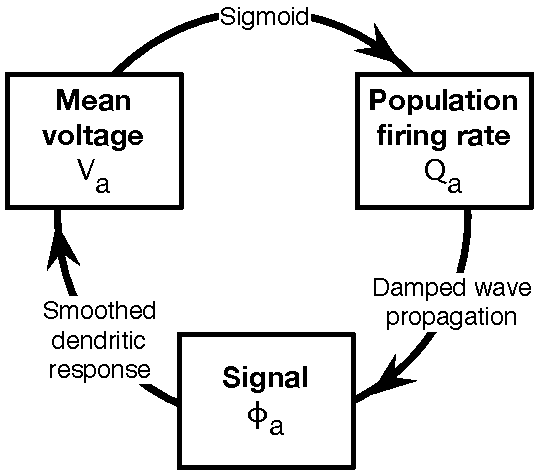
\includegraphics[width=0.40\columnwidth]{EIRS_cycle}
\caption{Schematic overview of the key dynamic quantities of neural field models, and the relationships between them.}
\label{fig:eirs_cycle}
\end{center}
\end{figure}

The most challenging part of applying neural field theory is the implementation of the numerical solver. Several factors contribute to making the numerical integration of neural field equations difficult. In particular, propagation delays between neural populations result in delay-differential equations that require special handling of temporal history. Further, propagation of neural fields according to a damped wave equation adds two dimensions to the system, and requires a relative sophisticated finite-differencing scheme that takes into account the geometry of the system. In addition, periodic boundary conditions must be correctly handled during the integration. 

We have developed NeuroField to provide a software package that solves the neural field equations for arbitrary neural populations, and contains library code for analysis and visualization, thus removing the barriers to quickly testing and analyzing neural field models. The software is designed to be easily extensible with basic C++ programming skills, making it simple to expand upon the basic model to include new phenomena. 

\section{Method and Results}
\label{sec:theory}

\subsection{Key features/Basic functions}
The essential role of NeuroField is to take as input a model and its initial conditions, and to output one or more time series corresponding to the result of integrating the neural field equations. A model is a specification of neural populations (amounting to defining their firing response to input from other populations including synapto-dendritic effects), and connections between the populations including how neural signals propagate through space. Sensory or other stimulus is implemented as a neural population that recieves no input from other populations, and has a pre-defined firing pattern. Integration of the neural field equations provides several quantities of interest. Most notably, the signals from populations can be associated with local field potentials (LFP) or EEG depending, and these predictions can be directly compared against experimental data. The soma potential or firing rate of the neural populations can be compared to individual neuron data. Changes to synaptic strength can be monitored when simulating neural plasticity. When simulating spatially extended populations, spatial correlations and patterns of activity can also be analyzed. 

The core of NeuroField is a C++ program that accept a human-readable plain text configuration file. The output from NeuroField is a plain text output file containing all of the requested simulation variables for each time step. The syntax of the output file has been designed to be simple to parse, and the NeuroField package includes reference parsers for Matlab and Python. These parsers may also help serve as a starting point for implementation of parsers other programming languages. 

There are a number of common ways to analyze the output from neural field models. First, plots of the time series are useful for directly viewing neural oscillations, evoked responses, seizures, monitoring plasticiity, and verifying stability. Second, calculation of the power spectrum, which is often compared to experimental EEG. This can also involve detection of multiple spatial modes of activity and incorporation of volume conduction, to account for effects introduced by electrodes in real-world recordings. Finally, spatial patterns of activity and propagation of waves of activity can be visualized on a surface plot. All of these basic analyses are included as Matlab programs in the NeuroField toolbox. 

\subsection{Data structures}
NeuroField is an object-oriented program where classes are used to encapsulate different components of the simulation. This structure makes it simple to write new components to customize parts of the simulation, that can be easily integrated into the rest of the simulation engine. An overview of the class structure is illustrated in Fig.~\ref{fig:class_hierarchy}. 

\begin{figure}[!h]
\tikzstyle{block} = [draw,text width=3em,text centered,minimum height=2em]
\tikzstyle{line} = [draw, -latex']    
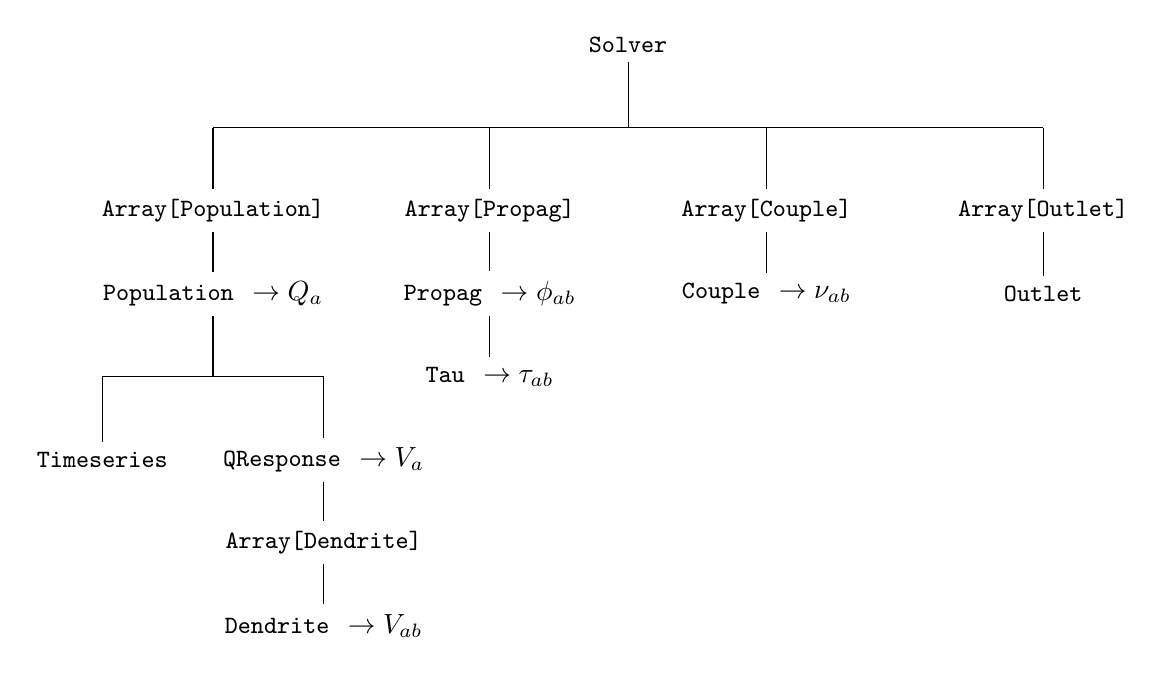
\begin{tikzpicture}[node distance = 3em, auto]
	\node[] (solver) {\type{Solver}};
    \node[below of=solver,node distance=3em] (vsolver) {};

	\node[left of=vsolver,node distance=5em] (vpropag) {};
	\node[left of=vpropag,node distance=10em] (vpop) {};
	\node[right of=vsolver,node distance=5em] (vcouple) {};
	\node[right of=vcouple,node distance=10em] (voutput) {};

    \draw (solver) -- (vsolver.center);
    \draw (vcouple.center) -- (voutput.center);
    \draw (vsolver.center) -- (vcouple.center);
    \draw (vpropag.center) -- (vpop.center);
    \draw (vsolver.center) -- (vpropag.center);


	\node[below of=vpropag] (apropag) {\type{Array[Propag]}};
	\node[below of=vpop]    (apop) {\type{Array[Population]}};
	\node[below of=vcouple] (acouple) {\type{Array[Couple]}};
	\node[below of=voutput] (aoutput) {\type{Array[Outlet]}};
    
    \draw (vpropag.center) -| (apropag);
    \draw (vpop.center) -| (apop);
    \draw (vcouple.center) -| (acouple);
    \draw (voutput.center) -- (aoutput);

	\node[below of=apropag] (propag) {\type{Propag} $\rightarrow \phi_{ab}$};
	\node[below of=apop]    (pop) {\type{Population} $\rightarrow Q_a$};
	\node[below of=acouple] (couple) {\type{Couple} $\rightarrow \nu_{ab}$};
	\node[below of=aoutput] (output) {\type{Outlet}};
    \draw (apropag) -- (propag);
    \draw (apop) -- (pop);
    \draw (acouple) -- (couple);
    \draw (aoutput) -- (output);

	\node[below of=pop,node distance=3em](vpop){};
	\node[left of=vpop,node distance=4em](vs){};
	\node[right of=vpop,node distance=4em](vq){};
    \draw (pop) |- (vpop);
    \draw (vpop.center) |- (vs.center);
    \draw (vpop.center) |- (vq.center);

	\node[below of=vs,node distance=3em](ts){\type{Timeseries}};
	\node[below of=vq,node distance=3em](qr){\type{QResponse} $\rightarrow V_a$};
    \draw (vs.center) -- (ts);
    \draw (vq.center) -- (qr);

	\node[below of=qr](adendrite){\type{Array[Dendrite]}};
	\node[below of=adendrite](dendrite){\type{Dendrite} $\rightarrow V_{ab}$};
    \draw (qr) -- (adendrite);
    \draw (adendrite) -- (dendrite);

	\node[below of=propag,node distance=3em](tau){\type{Tau} $\rightarrow \tau_{ab}$};
	\draw(propag)--(tau);
\end{tikzpicture}
\caption{Schematic diagram showing key NeuroField objects, their hierarchical relationships, and their principal associated dynamic quantities.}
\label{fig:class_hierarchy}
\end{figure}

The high-level classes \texttt{Solver} and \texttt{Array} serve as containers to drive the simulation, and to store collections of simulation elements, respectively. The \texttt{outlet} object serves as a modular container for writing variables into the output file. Creating an \texttt{outlet} object enables any variable (including new user-defined quantities) to be included in the output. 

The main objects (\texttt{Couple}, \texttt{Dendrite}, \texttt{Qresponse}, \texttt{Population} and \texttt{Propag}) are each responsible for one part of the neural field model. 
\begin{align}
	P &= \nu_{ab}\phi_{ab}, & \mathtt{Couple}\\
	D_{ab}V_{ab} &= P, & \mathtt{Dendrite}\\
	Q_a &= S_a \big[\sum_b V_{ab} \big], & \mathtt{QResponse/Pop}\\
	\mathcal{D}_{ab}\phi_{ab} &= Q_b,&  \mathtt{Propag}
\end{align}

\begin{figure}
\tikzstyle{pop_style} = [rectangle, draw, text width=6em, text centered, minimum height=4em]
\tikzstyle{couple_style} = [rectangle, draw, text width=6em, text centered, minimum height=4em,fill=gray!10]
\tikzstyle{line} = [draw, -latex']    
\begin{tikzpicture}[node distance = 2.7cm, auto]
    \node[pop_style] (qresponse) {\texttt{QResponse}\\$V_a \rightarrow Q_a$};
    \node[pop_style,right of=qresponse] (pop) {\texttt{Population}\\$Q_b$};
    \node[couple_style,right of=pop] (propag) {\texttt{Propag}\\ $Q_b \rightarrow \phi_{ab}$};
    \node[couple_style,right of=propag] (couple) {\texttt{Couple}\\$\phi_{ab} \rightarrow \nu_{ab}\phi_{ab}$};
    \node[couple_style,right of=couple] (dendrite) {\texttt{Dendrite}\\$\nu_{ab}\phi_{ab}\rightarrow V_{ab}$};
    \draw[line] (pop) -- (propag);
    \draw[line] (propag) -- (couple);
    \draw[line] (couple) -- (dendrite);
    \draw[line] (qresponse) -- (pop);
\end{tikzpicture}
\caption{Schematic diagram showing the relationship between fundamental NeuroField objects. The white blocks conceptually relate to neural populations, and the shaded blocks relate to connections.}
\label{fig:components}
\end{figure}

\subsubsection{Populations}
A \texttt{Population} object represents a neural population, which is primarily characterized by a firing rate. A stimulus population is one that has no incoming connections, instead firing according to a pre-programmed selection (e.g., white noise, or pulsed activity). Other populations recieve connections from of other populations, which are specified as a set of \texttt{Couple} objects. Each population contains two subsidiary objects, an array of \texttt{Dendrite} objects (one for each \texttt{Couple}), and a \texttt{QResponse}. The signal arriving through a \texttt{Couple} object is passed to a corresponding \texttt{Dendrite} which implements the synaptodendritic effects in Eq.~\eqref{eq:dendrite}. The contribution $V_{ab}$ from each presynaptic population is then summed to provide the soma potential $V_a$. The population's \texttt{QResponse} object then provides the implementation of Eq.~\ref{eq:sigmoid} which calculates the population's resulting firing rate. Another common alternative for the firing response is a linear function, which is suitable for small perturbations to a steady state. These behaviours are all specified within the \texttt{QResponse} object. 

Finally, populations may be further customized to provide additional functionality. One notable example is the inclusion of bursting, which introduces two new dynamic properties of the population that are integrated at each time step. NeuroField includes a basic fourth-order Runge-Kutta integrator that is suitable for these types of additions. The modular nature of NeuroField enables this integrator to be easily substituted with a user-defined function. 

\todo[inline]{More from XL about this}

\subsubsection{Propagators}
The neural field generated by a population propagates according to Eq.~\ref{eq:wave}, which is encapsulated in a \texttt{Propag} object. There are as many \texttt{Propag} objects as there are connections in the model. There are three fundamental possibilities for the propagator. First, the propagator may simply be a direct mapping, with $\mathcal{D}_a(\mathbf{r},t) = 1$. This is commonly used for short-range local connections. Second, for spatially localized activity we can include only the time derivaties in Eq.~\ref{eq:wave}, which gives a \emph{harmonic} propagator. Finally, we can consider the full expression in Eq.~\ref{eq:wave}, which is the full wave propagator.

Much of the complexity of NeuroField lies in the solution to the wave equation. NeuroField uses an explicit finite difference (9 point) algorithm on a regular square grid with periodic boundary conditions to solve the wave equation. Implementation of the periodic boundary conditions requires that the 9 point stencil correctly wrap around the edges of the grid at every time step. Correct, efficient implementation of this step tends to be the biggest hurdle to implementing a neural field model. 

\todo[inline]{Do we have a derivation or something for the actual stencil equation? (FELIX)}

\begin{figure}[!b]
\begin{center}
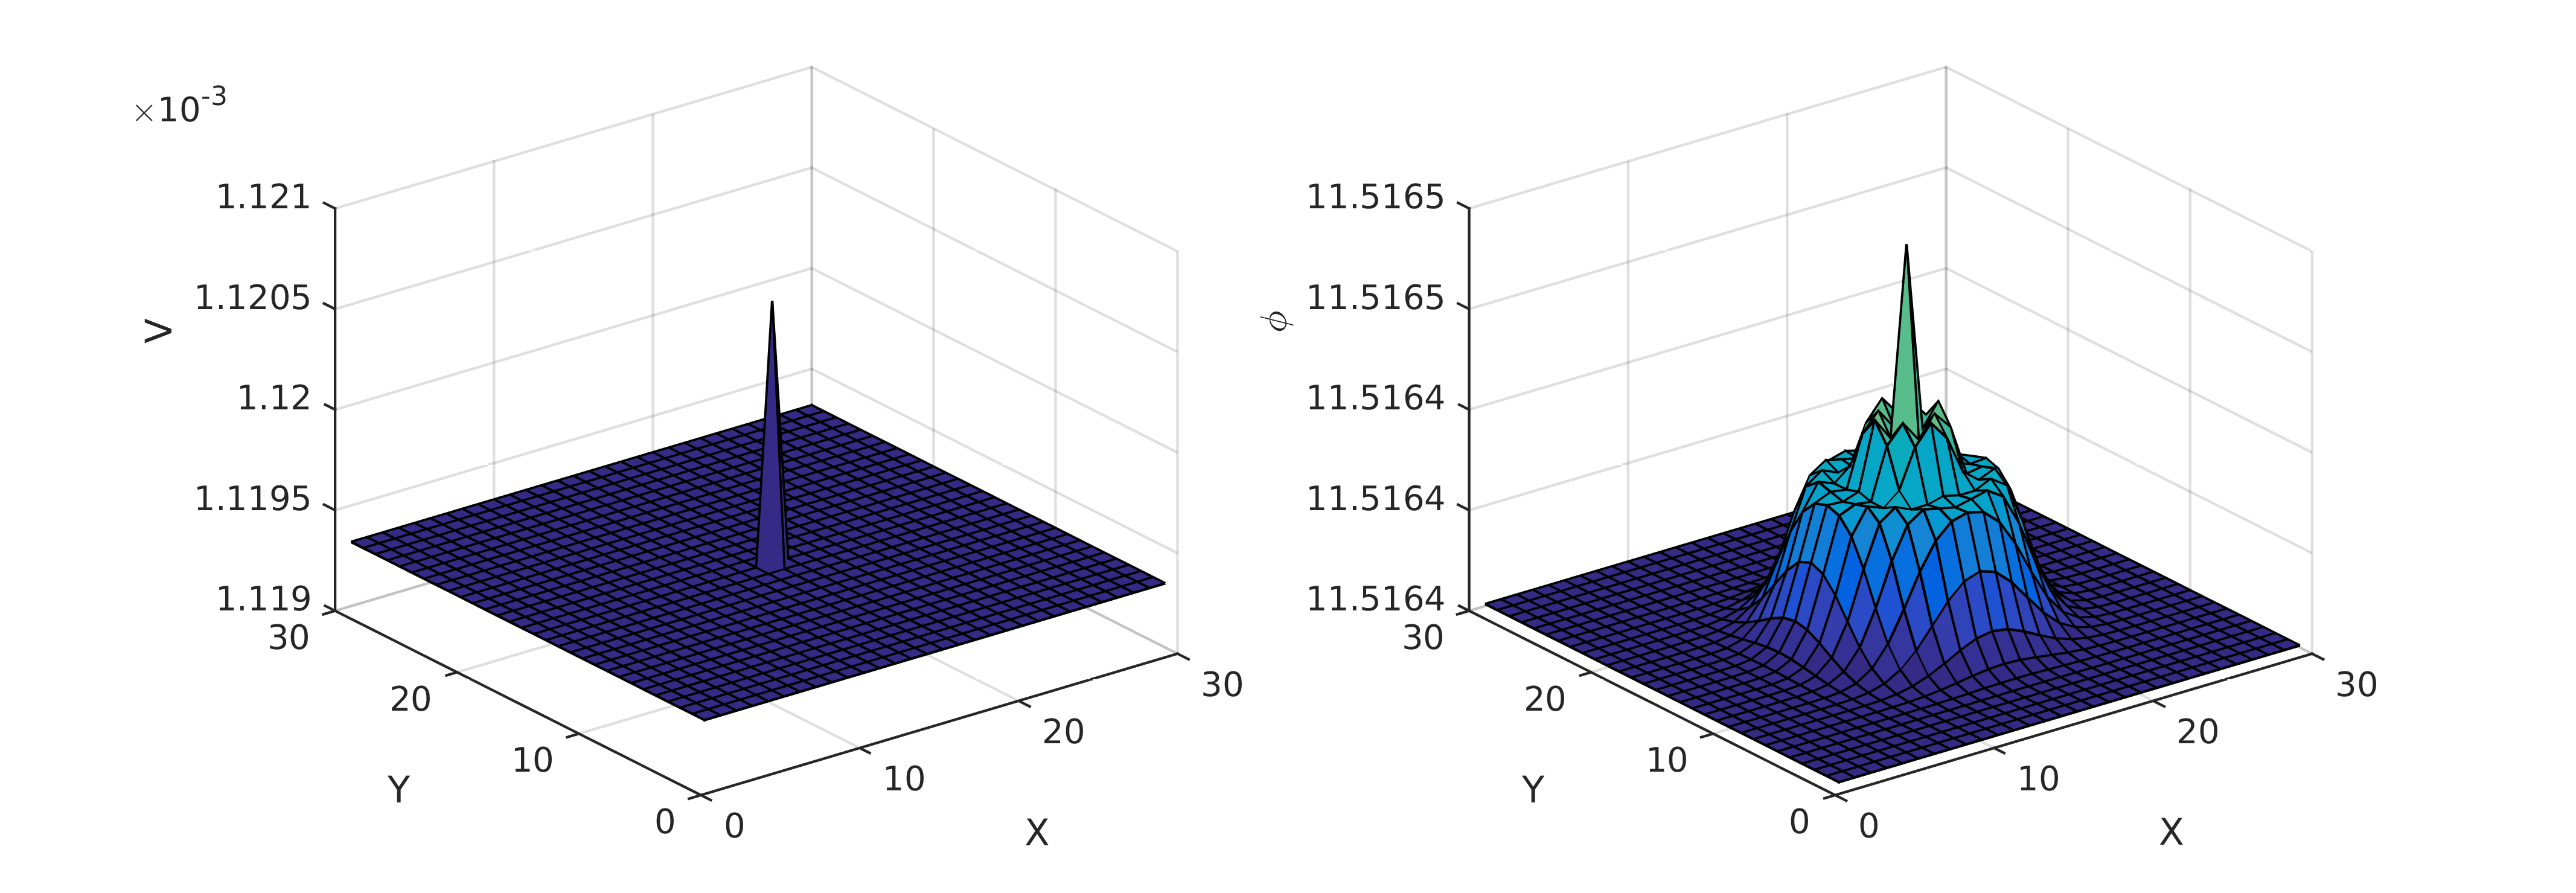
\includegraphics[width=1\columnwidth]{wave_comparison}
\caption{Effect of wave propagation in a single-population model. The stimulus is a single short pulse at the center node. The left panel shows population voltage $V_a$, which shows the spatial localization of the input signal. The right panel shows the signal $\phi_a$ after wave propagation.}
\label{fig:wave_comparison}
\end{center}
\end{figure}

The propagator also takes into account the spatial geometry of the problem. By default, NeuroField solves the wave equation on a flat grid. However, by considering a wave propagator of the form $\mathcal{D}_a(\mathbf{r},\mathbf{r'},t)$, arbitrary metric tensors may be implemented. This type of propagator enables wave propagation on curved surfaces, which may be as simple as a sphere or as detailed as a surface based on structural MRI. 

\todo[inline]{More from XL/John about this}

Finally, the propagator object also encapsulates any time delays, which typically arise due to spatial separation of neural populations (for example, between cortical and thalamic populations). By storing the time delay internally in the \texttt{Propag} object, all other parts of the simulation are able to simply query the \texttt{Propag} to obtain $\phi_b$, and the \texttt{Propag} will return the retarded value where applicable. Thus customizing other parts of the model requires no special handling of time delays. The delays may also vary spatially, so that different parts of the system have different time delays. 

\subsubsection{Couples}
The coupling strength $\nu_{ab}$ scales the incoming signals, weighting the contribution from different presynaptic sources. The strength of the synapse is stored in a \texttt{Couple} object. Typically the strength is constant, reflecting the number and strength of the relevant synaptic connections. However, modulation of the coupling strengths forms the basis of neural plasticity. In NeuroField, this is achieved by modifying the \texttt{Couple} to take into account time-varying connections. We have used this functionality in previous studies to model a wide range of plasticity effects including spike-timing dependent plasticity (STDP) and calcium dependent plasticity (CaDP). 

\todo[inline]{More from Felix about this}

\subsubsection{Input and output}
NeuroField input and output are written in plain text files, which are human readable and simple to construct and parse programatically. An simple configuration file is shown in Fig.~\ref{fig:config_text}.  

The configuration file first starts with a specification of the simulation duration and time step. The total number of nodes is specified, and assumed to correspond to a square grid - in this case, 30x30 nodes. It is also possible to specify a rectangular grid at this point. 

Next, a list of connections is provided, formatted as a human-readable connection matrix. Each connection is assigned a number at this point. The dimension of the matrix corresponds to the number of populations being simulated, and the number of nonzero entries in the matrix corresponds to the number of couplings, propagators and dendrites.

Following the connection matrix is a detailed specification for each population. The spatial grid resolution is determined automatically based on the number of nodes and the physical dimensions of the population. The Courant condition for numerical stability is automatically checked. The firing response is specified for each population, with parameters delegated to the appropriate \texttt{QResponse} object. The parameters for each afferent dendrite are specified at this point as well. Stimulus populations have no dendrites. Instead, the stimulus is specified by a \texttt{TimeSeries} object, a container that returns a firing rate as a function of time. In Fig.~\ref{fig:config_text}, the stimulus is of type \texttt{Pulse}, and acts at only a single node of the simulation. Different stimuli can be applied at different times, and multiple stimulus populations can be used to investigate the effect of superimposing stimuli. 

For each connection, the propagator and coupling type need to be specified. In Fig.~\ref{fig:config_text}, one of the propagators is given by the wave equation, and the other is a direct mapping. The time delay, axonal range, and damping rate are all specified independently for each propagator. 

The final block in the configuration file selects the output from NeuroField. The output can include all of the nodes, or a user-defined subset of nodes. The start of the output can be delayed to remove transients from the output. To ensure numerical stability, the equations need to be integrated with a very small time step (e.g., $1\times10^{-4}$\,s$=10000$\,Hz). This is much smaller than typically required for analysis; EEG is typically sampled at just 500\,Hz or less. To reduce file size and make handling the output less computationally intensive, an output sampling interval can be specified, downsampling the output from NeuroField. 

\begin{figure}[!htbp]
\begin{center}
\begin{lstlisting}
Time: 0.15 Deltat: 0.0001
Nodes: 900

    Connection matrix:
From:  1  2 
To 1:  1  2  
To 2:  0  0  


Population 1: Excitatory
Length: 0.5
Q: 10.98
Firing: Sigmoid - Theta: 0.01292 Sigma: 0.0038 Qmax: 340
 Dendrite 1: alpha: 83.33333333 beta: 769.2307692
 Dendrite 2: alpha: 83.33333333 beta: 769.2307692

Population 2: Stimulation
Length: 0.5
 Stimulus: Pulse - Onset: 0 Node: 465 Amplitude: 1 Width: 1e-3 

Propag 1: Wave - Tau: 0 Range: 0.2 gamma: 30
Propag 2: Map - Tau: 0

Couple 1:  Map - nu: 1e-4
Couple 2:  Map - nu: 1e-4

Output: Node: All Start: 0 Interval: 1e-4
Population: 1
Dendrite:  
Propag: 1
Couple:  
\end{lstlisting}
\caption{Example config file from NeuroField, for a simple system consisting of one neural population, and a stimulus. This configuration was used to generate Fig.~\ref{fig:wave_comparison}.}
\label{fig:config_text}
\end{center}
\end{figure}

\todo[inline]{Stuff about the output file}

\begin{figure}[!b]
\begin{center}
\begin{lstlisting}
    Time  |             Pop.1.V  |        Dendrite.1.V  |
          |                   1  |                   1  |
5.00e-03  | -1.020386100923e-03  |  2.589927678839e-02  |
1.00e-02  | -1.020386100890e-03  |  2.589927678842e-02  |
\end{lstlisting}
\caption{Example output from NeuroField, showing two time series from different parts of the system. The plain text file contains a row for each time, and a column for each quantity requested.}
\label{fig:output_text}
\end{center}
\end{figure}

\subsection{Visualization and analysis}

\subsubsection{Helper scripts}
NeuroField is packaged with several helper scripts written in MATLAB to assist with running, analyzing and visualizing models. 

\subsubsection{Reading output files}
nf\_read() allows users to parse the output file from NeuroField into a MATLAB struct object.
nf\_grid reshapes the output for handling matrices. 

\subsubsection{Writing config files}
nf\_eirs() demonstrates writing a configuration file, running it with nf\_run(), and then reading it with nf\_read(). This demonstrates a complete MATLAB-based toolchain for using NeuroField.

\subsubsection{Calculating power spectra}
The power spectrum can be obtained by FFT, but correct normalization and calculation of the power spectrum including multiple spatial modes can be challenging to implement. We have implemented a 3D FFT algorithm that correctly normalizes the output and includes volume conduction effects that selective attenuate spatial modes depending on their wavenumber. The result can be directly compared to analytical predictions.

\begin{figure}[!b]
\begin{center}
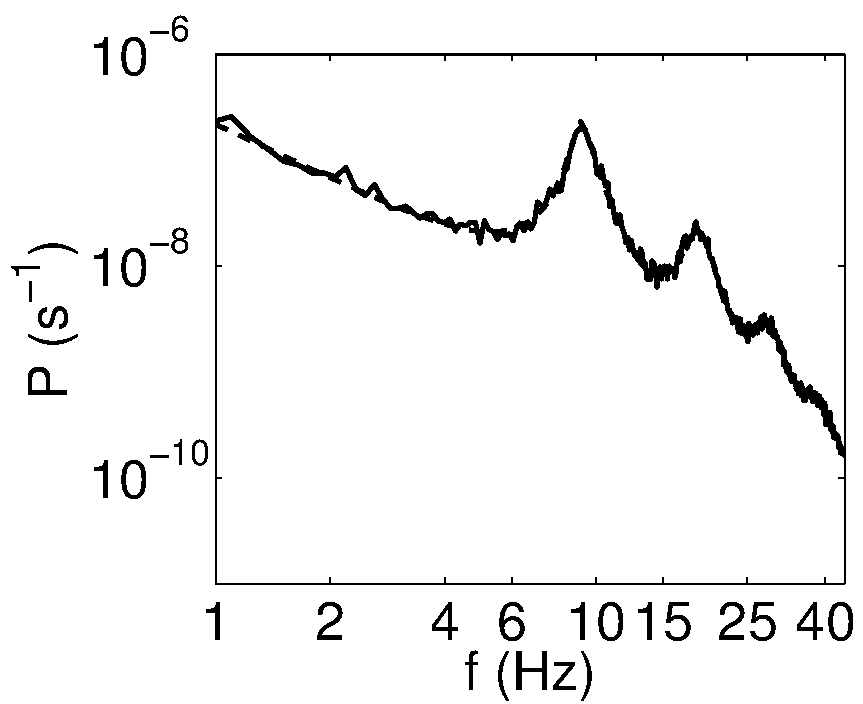
\includegraphics[width=0.80\columnwidth]{corticothalamic_comparison}
\caption{Comparision of linear analytic spectrum with the power spectrum computed using the NeuroField package analysis tools.}
\label{fig:ct_spectrum}
\end{center}
\end{figure}

\subsubsection{Visualizing output}
The nf\_extract() function makes it easy to select data for plotting from a NeuroField object.  
nf\_movie can plot an animation of the output

\clearpage

\section{Results}

In this section, we present examples of NeuroField applied to recent research.

\subsection{Corticothalamic model (Romesh)}

NeuroField has been extensively tested with a recent neural field corticothalamic model of the brain \citep{Robinson2005,Rowe2004413,PhysRevE.63.021903,PhysRevE.65.041924,Robinson:04aa} that we have previously used to investigate the alpha rhythm \citep{PhysRevE.68.021922,PhysRevE.70.011911}, age-related changes to the physiology of the brain \citep{VanAlbada2010}, evoked response potentials \citep{Rennie2002,ker11}, seizures \citep{Breakspear2006}, and many other phenomena. 

\begin{figure}[!b]
\begin{center}
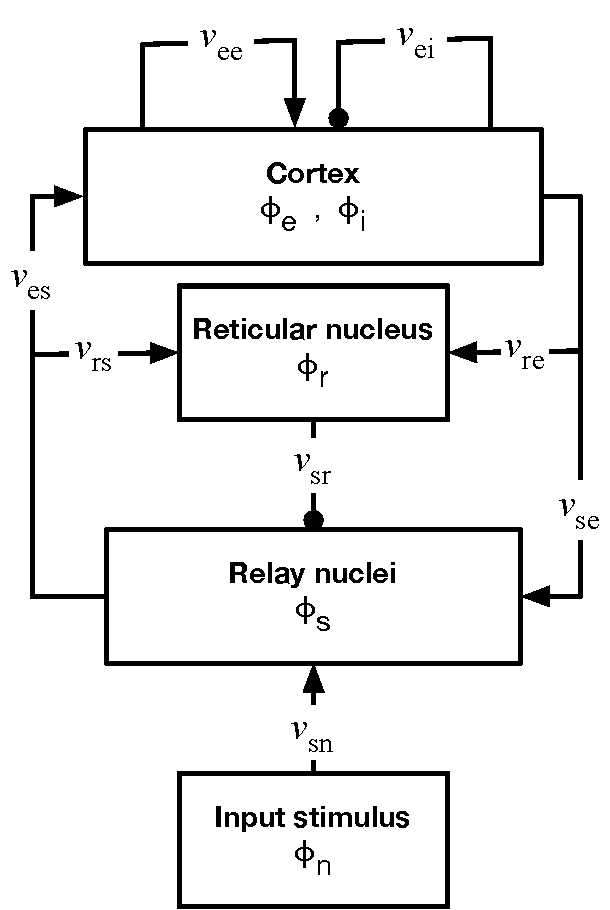
\includegraphics[width=0.40\columnwidth]{EIRS_clean}
\caption{Schematic overview of the corticothalamic model.}
\label{fig:ct_schematic}
\end{center}
\end{figure}

The structure of the model is shown in Fig.~\ref{fig:ct_schematic}. Much of our work is in the linear regime and utilizes analytic results for small perturbations to steady states. Steady states can be obtained by setting the differential operators \eqref{eq:dendrite} and \eqref{eq:wave} to unity, and solving for the the steady state firing rate $\phi_e^{(0)}$ \cite{Robinson:04aa}
\begin{align}
	\label{eqn:ve_root}
	\begin{split}
	S^{-1}&(\phi_e^{(0)})-(\nu_{ee}+\nu_{ei})\phi_e^{(0)} = \\ &\nu_{es}S\left\{\nu_{se}\phi_e^{(0)}+\nu_{sr}S\left[\nu_{re}\phi_e^{(0)}+(\nu_{rs}/\nu_{es})\left(S^{-1}(\phi_e^{(0)})-(\nu_{ee}+\nu_{ei})\phi_e^{(0)}\right)\right]+\nu_{sn}\phi_n^{(0)}\right\}, 
\end{split}\\[16pt]
%	\label{eqn:ve_root_numeric}
%	\begin{split}
	V_e^{(0)}&-(\nu_{ee}+\nu_{ei})S(V_e^{(0)})=\\ &\nu_{es}S\left\{\nu_{se}S(V_e^{(0)})+\nu_{sr}S\left[\nu_{re}S(V_e^{(0)})+(\nu_{rs}/\nu_{es})\left(V_e^{(0)}-(\nu_{ee}+\nu_{ei})S(V_e^{(0)})\right)\right]+\nu_{sn}\phi_n^{(0)}\right\},
%\end{split}
\end{align}
where $S^{-1}$ denotes the inverse sigmoid function. To linearize the model, we consider a Taylor expansion of the sigmoid around the steady state:
\begin{align}
Q_a(\mathbf{r},t) = Q_a^{(0)} + S'\left(V_a^{(0)}\right) \left[V_a(\mathbf{r},t)-V_a^{(0)}\right] \\
+ \frac{S''\left(V_a^{(0)}\right)}{2!} \left[V_a(\mathbf{r},t)-V_a^{(0)}\right]^2 \cdots ,
\end{align}
which can be written in terms of a perturbation by relabeling $Q_a-Q_a^{(0)} \rightarrow Q_a $, $V_a-V_a^{(0)} \rightarrow V_a$, yielding

\begin{align}
\label{eqn:q_series}
Q_a(\mathbf{r},t) &= \rho_a^{(1)} V_a(\mathbf{r},t) + \frac{\rho_a^{(2)}}{2} V_a(\mathbf{r},t)^2 \cdots .
\end{align}


where $\rho_a^{(n)} = S^{(n)}\left(V_a^{(0)}\right)$ and $S^{(n)}$ is the $n$th derivative of the sigmoid function at the steady state value of $Q_a$. 

However, some phenomena are strongly nonlinear, and these must be solved by numerical integration. We have used NeuroField to model results relating to seizures \citep{Roberts2008}, visually evoked potentials \citep{Roberts2012a}, and sleep spindles \citep{Abeysuriya2013,Abeysuriya2013a}. 



\begin{align}
\label{eqn:power_sum}
P(\omega) &= \sum_{m = -\infty}^{\infty}\sum_{n = -\infty}^{\infty} \Delta k_x \Delta k_y |T(\mathbf{k},\omega)|^2||\phi_n(\mathbf{k},\omega)|^2F(k)\\
k^2 &=  \left( \frac{2\pi m}{L_x} \right)^2 + \left( \frac{2\pi n}{L_y}\right)^2 
\end{align}
where the size of the two-dimensional rectangular cortex is $L_x \times L_y$. 

\begin{align}
F(k) &= e^{-k^2/k_0^2},
\end{align}


Prediction of the EEG power spectrum involves two additional steps - first, summation over 
\begin{figure}[!b]
\begin{center}
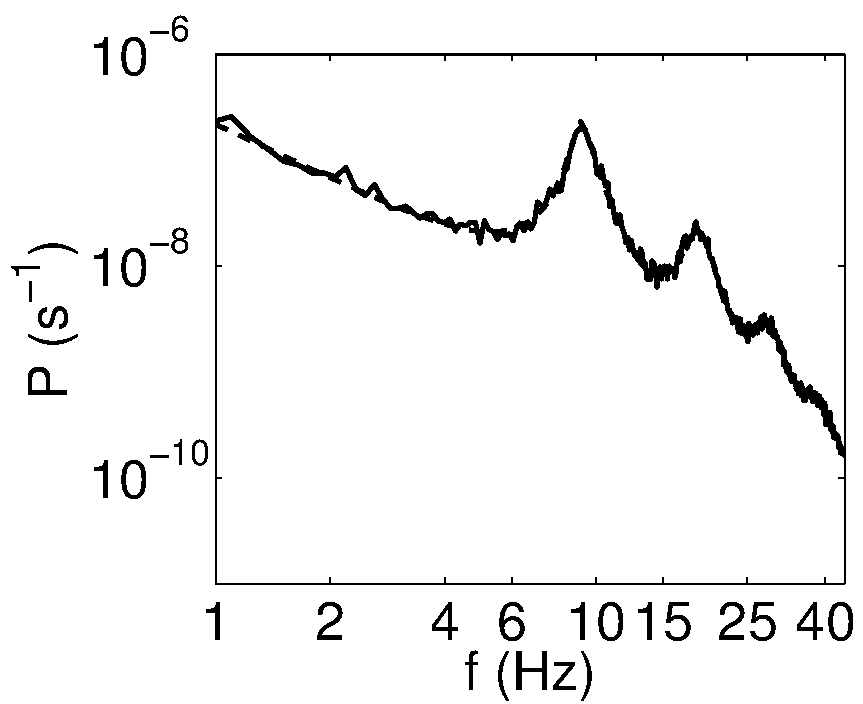
\includegraphics[width=0.40\columnwidth]{corticothalamic_comparison}
\caption{Wake EC, same params as already published}
\label{fig:ct_spectrum_1}
\end{center}
\end{figure}

\begin{itemize}
	\item Sleep spindles
	\item Wake alpha peak
	\item Volume conduction
\end{itemize}

\subsection{Plasticity (Felix)}

\subsection{Bursting (XL)}

\subsection{Seizures (XL)}

\section{Discussion}
\label{sec:discussion}

We have developed NeuroField to provide an extensible, reliable framework for integrating nonlinear delay differential equations including spatial propagation. NeuroField is aimed for use by researchers who have constructed neural field models of the brain that require numerical integration. In this section, we review some usage and performance considerations.

\subsection{White noise stimulus}
\begin{itemize}
	\item White noise requires stocastic DE integrator, effectively Euler (FELIX)
	\item Noise amplitude depends on grid resolution as this affects the possible bandwidth. Similar features depend on frequency domain power so noise needs to be normalized correctly (ROMESH)
\end{itemize}

\subsection{Performance}

\begin{itemize}
\item Some numbers about the runtime and memory requirements of NeuroField (FELIX)
\item Note that the memory requirements scale with the grid size, and the grid size depends on Lx and the propagator lengths (automatically enforced) (FELIX)
\item Also that the delays in the system cause O(n) increases in memory usage (FELIX)
\end{itemize}

\todo[inline]{Additional considerations?}

\section{Acknowledgements}
\label{sec:acknowledgements}
This work was supported by the Australian Research Council, National Health and Medical Research Council (through the Center for Integrated Research and Understanding of Sleep), and the Westmead Millennium Institute.

\section{References}
\bibliographystyle{complex_vancouver}
\bibliography{neurofield}

\end{document}

%% References
%%
%% Following citation commands can be used in the body text:
%%
%%  \citet{key}  ==>>  Jones et al. (1990)
%%  \citep{key}  ==>>  (Jones et al., 1990)
%%
%% Multiple citations as normal:
%% \citep{key1,key2}         ==>> (Jones et al., 1990; Smith, 1989)
%%                            or  (Jones et al., 1990, 1991)
%%                            or  (Jones et al., 1990a,b)
%% \citep{key} is the equivalent of \citet{key} in author-year mode
%%
%% Full author lists may be forced with \citet* or \citep*, e.g.
%%   \citep*{key}            ==>> (Jones, Baker, and Williams, 1990)
%%
%% Optional notes as:
%%   \citep[chap. 2]{key}    ==>> (Jones et al., 1990, chap. 2)
%%   \citep[e.g.,][]{key}    ==>> (e.g., Jones et al., 1990)
%%   \citep[see][pg. 34]{key}==>> (see Jones et al., 1990, pg. 34)
%%  (Note: in standard LaTeX, only one note is allowed, after the ref.
%%   Here, one note is like the standard, two make pre- and post-notes.)
%%
%%   \citealt{key}          ==>> Jones et al. 1990
%%   \citealt*{key}         ==>> Jones, Baker, and Williams 1990
%%   \citealp{key}          ==>> Jones et al., 1990
%%   \citealp*{key}         ==>> Jones, Baker, and Williams, 1990
%%
%% Additional citation possibilities
%%   \citeauthor{key}       ==>> Jones et al.
%%   \citeauthor*{key}      ==>> Jones, Baker, and Williams
%%   \citeyear{key}         ==>> 1990
%%   \citeyearpar{key}      ==>> (1990)
%%   \citetext{priv. comm.} ==>> (priv. comm.)
%%   \citenum{key}          ==>> 11 [non-superscripted]
%% Note: full author lists depends on whether the bib style supports them;
%%       if not, the abbreviated list is printed even when full requested.
%%
%% For names like della Robbia at the start of a sentence, use
%%   \Citet{dRob98}         ==>> Della Robbia (1998)
%%   \Citep{dRob98}         ==>> (Della Robbia, 1998)
%%   \Citeauthor{dRob98}    ==>> Della Robbia


%% References with bibTeX database:

%% Authors are advised to submit their bibtex database files. They are
%% requested to list a bibtex style file in the manuscript if they do
%% not want to use elsarticle-harv.bst.

%% References without bibTeX database:

% \begin{thebibliography}{00}

%% \bibitem must have one of the following forms:
%%   \bibitem[Jones et al.(1990)]{key}...
%%   \bibitem[Jones et al.(1990)Jones, Baker, and Williams]{key}...
%%   \bibitem[Jones et al., 1990]{key}...
%%   \bibitem[\protect\citeauthoryear{Jones, Baker, and Williams}{Jones
%%       et al.}{1990}]{key}...
%%   \bibitem[\protect\citeauthoryear{Jones et al.}{1990}]{key}...
%%   \bibitem[\protect\astroncite{Jones et al.}{1990}]{key}...
%%   \bibitem[\protect\citename{Jones et al., }1990]{key}...
%%   \harvarditem[Jones et al.]{Jones, Baker, and Williams}{1990}{key}...
%%

% \bibitem[ ()]{}

% \end{thebibliography}

%%
%% End of file `elsarticle-template-harv.tex'.
